%% chapters/chapter_1.tex
%%
%% Copyright 2017 Evandro Coan
%% Copyright 2012-2014 by abnTeX2 group at http://abntex2.googlecode.com/
%%
%% This work may be distributed and/or modified under the
%% conditions of the LaTeX Project Public License, either version 1.3
%% of this license or (at your option) any later version.
%% The latest version of this license is in
%%   http://www.latex-project.org/lppl.txt
%% and version 1.3 or later is part of all distributions of LaTeX
%% version 2005/12/01 or later.
%%
%% This work has the LPPL maintenance status `maintained'.
%%
%% The Current Maintainer of this work is the Evandro Coan.
%%
%% The last Maintainer of this work was the abnTeX2 team, led
%% by Lauro César Araujo. Further information are available on
%% https://www.abntex.net.br/
%%
%% This work consists of a bunch of files. But originally there were 2 files
%% which are renamed as follows:
%% Deleted the `abntex2-modelo-img-marca.pdf`
%% Renamed the `abntex2-modelo-include-comandos.tex, v-1.9.2 laurocesar` to `chapters/chapter_1.tex`
%%
% ---
% Este capítulo, utilizado por diferentes exemplos do abnTeX2, ilustra o uso de
% comandos do abnTeX2 e de LaTeX.
% ---

% The \phantomsection command is needed to create a link to a place in the document that is not a
% figure, equation, table, section, subsection, chapter, etc.
%
% When do I need to invoke \phantomsection?
% https://tex.stackexchange.com/questions/44088/when-do-i-need-to-invoke-phantomsection
\phantomsection


% Is it possible to keep my translation together with original text?
% https://tex.stackexchange.com/questions/5076/is-it-possible-to-keep-my-translation-together-with-original-text
\chapter{Fundamentação Teórica}
\label{cap:fundamentacao_teorica}

% \newpage

Esta seção apresenta a fundamentação teórica sobre o processador \manycore \mppa e o \fw PSkel, sua adaptação utilizada nesse trabalho.

\section{MPPA-256}
\label{sec:mppa}

O \mppa é um processador \manycore desenvolvido pela empresa francesa
Kalray. Esse processador possui 256 núcleos e usuário e 32 núcleos de sistema para processamento a 400 MHz. Esses núcleos estão distribuídos entre 16 \textit{clusters} de computação e 4 \textit{clusters} de \textit{Input/Output}(\io), que se comunicam através de NoCs de dados e controle. O processador utilizado no desenvolver deste projeto de pesquisa possui uma memória global de baixa potência (LPDDR3) de 2GB conectada a um dos susistemas de \io. A arquitetura do \mppa é ilustrada na Figura~\ref{fig:mppaOverall}. Cada cluster de computação tem os seguintes componentes:

\begin{itemize}
    \item 16 núcleos chamados de \textit{Processing Elements} (\pes), que são responsáveis por executar as \textit{threads} de usuário (uma \textit{thread} por \pe), e não pode ser interrompida ou preemptada;
    
    \item um \textit{Resource Manager} (\rman), responsável por executar o sistema operacional e gerenciar a comunicação;
    
    \item uma memória compartilhada de baixa latência de 2MB, que permite um grande banda e fluxo e dados e controle entre os \pes presentes no mesmo \textit{cluster} de computação; e
    
    \item dois controladores de NoC, um para dados e outro para controle.
    
\end{itemize}

\begin{figure}
    \centering
    \caption{Arquitetura do MPPA-256.}
    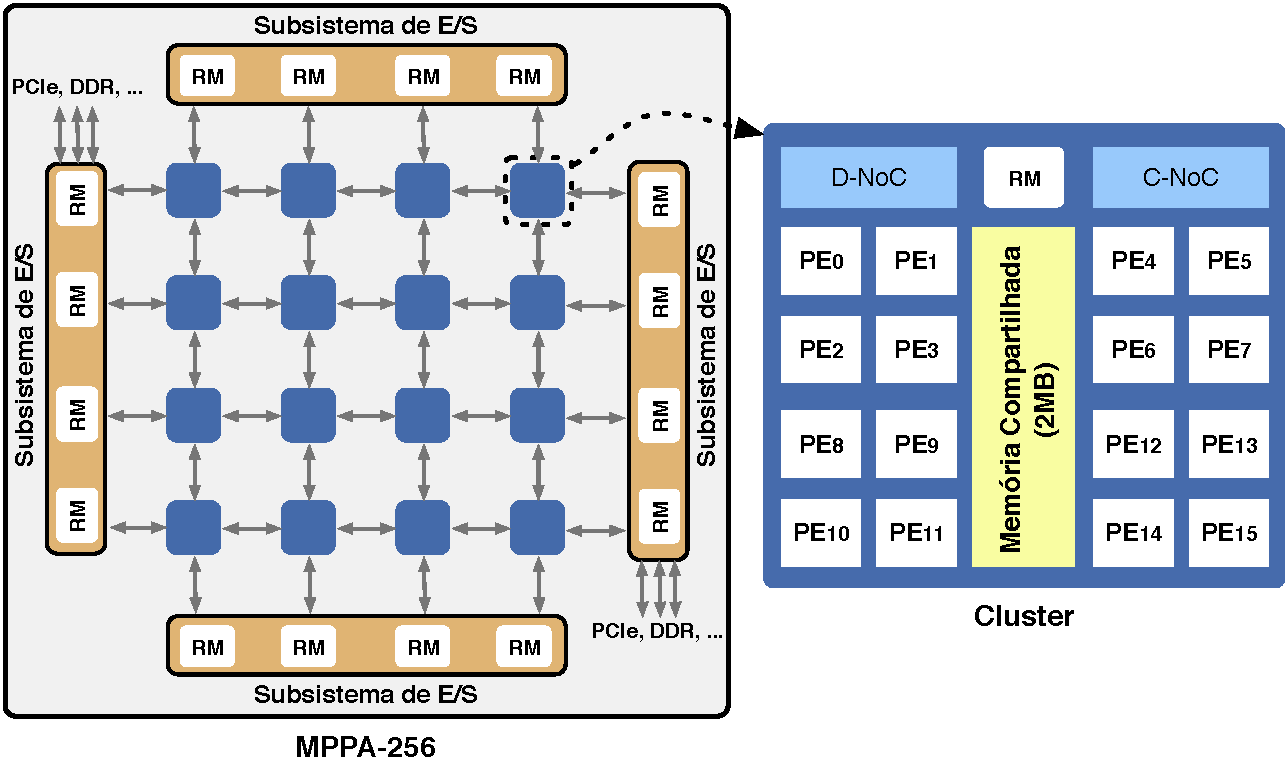
\includegraphics[width=0.5\textwidth]{figs/mppa-overview.pdf} \\
    Fonte: ...
    \label{fig:mppaOverall}
\end{figure}

\begin{figure}
    \centering
    \caption{O padrão estêncil.}
    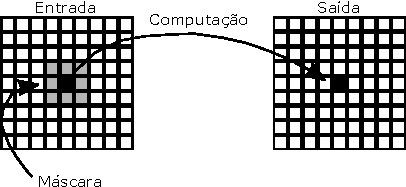
\includegraphics[width=0.5\textwidth]{figs/stencilComputation.pdf} \\
    Fonte: ...
    \label{fig:stencil}
\end{figure}



Trabalhos anteriores mostraram que desenvolver aplicações paralelas otimizadas
para o \mppa é um grande desafio~\cite{francesquini:hal-01092325} devido a alguns
fatores importantes, tais como: o modelo de memória distribuída presente no
\mppa, a capacidade de memória dentro do \textit{chip} e a comunicação explícita
através da \noc. Mais detalhes sobre esses desafios são apresentados em
~\cite{wscad2017}.

\section{Padrão estêncil e PSkel}
\label{sec:pskel}

O padrão estêncil, ilustrado pela Figura~\ref{fig:stencil}, funciona da
seguinte forma. Para cada elemento de
uma estrutura $n$-dimensional é computado um novo valor relativo aos vizinhos do
elemento atual. Os vizinhos de um elemento são determinados pela máscara da
computação. Por fim, cada novo valor computado é atribuído à sua célula
respectiva em uma estrutura $n$-dimensional de saída. Em aplicações
estêncil iterativas, a estrutura de saída é utilizada como
estrutura de entrada de uma nova iteração da aplicação.

O \pskel é um \fw de programação em alto nível para aplicações baseadas no
padrão estêncil, baseado no conceito de esqueletos paralelos, oferecendo suporte para a execução dessas aplicações em
ambientes heterogêneos, incluindo \cpu e \gpu. \pskel oferece um interface única de programação, desacoplada do \textit{back-end} de execução, permitindo que o usuário se preocupe apenas em implementar o \textit{kernel} estêncil que descreve a computação, enquanto o \fw fica responsável pela tradução das abstrações descritas para código paralelo de baixo nível em C++, gestão de memória e transferência de dados, tudo isso de forma transparente paar o usuário~\cite{CPE:CPE3479}.


\section{PSkel-MPPA}
\label{sec:pskel-mppa}

A adaptação PSkel-MPPA, é uma adaptação do \pskel proposta por~\cite{wscad2017}, ela faz uso de uma \api similar à POSIX \ipc para comunicação, e será tratada como \ipc no decorrer deste relatório. Nela, são utilizados portais de comunicação para o envio de dados e o método de \textit{strides}  para gerenciar explicitamente o envio e recebimento de \textit{tiles}. Essa adaptação possíbilita o uso do \fw PSkel com o processador \manycore \mppa.
